\documentclass{article}
\usepackage[dblblindworkshop,nonanonymous]{neurips_2026}
\usepackage[utf8]{inputenc}
\usepackage[T1]{fontenc}
\usepackage{amsmath,amssymb,booktabs,graphicx,microtype,url,longtable,placeins}
\usepackage[hidelinks]{hyperref}
\usepackage{tikz}
\usetikzlibrary{arrows.meta,positioning,fit}
\workshoptitle{Physical World AI: Geometry, Characteristics, and Multimodal Sensing}
\title{JEPA-FORGE: Auditable Context--Target Selection\\for Predictive Representations}
\author{Anonymous Authors}
\hypersetup{pdftitle={JEPA-FORGE: Auditable Context-Target Selection for Predictive Representations},pdfauthor={},pdfsubject={Anonymous workshop draft; not submitted},pdfkeywords={predictive representations, task selection, sensor trajectories, evaluation}}
\makeatletter
\renewcommand{\@noticestring}{Anonymous workshop draft for PhysWorldAI, NeurIPS 2026 (Atlanta). Not submitted.}
\makeatother
\newcommand{\jepa}{JEPA-FORGE}
\newcommand{\sg}{\operatorname{sg}}
\newcommand{\relu}{\operatorname{ReLU}}
\newcommand{\ExtTasks}{27}
\newcommand{\ExtSplits}{81}
\newcommand{\ExtRuns}{1044}
\newcommand{\ExtCheckpoints}{1284}
\newcommand{\ExtPolicyWins}{10}
\newcommand{\ExtShortWins}{16}
\newcommand{\ExtTreesWins}{5}
\newcommand{\ExtLinearWins}{10}
\newcommand{\ExtSupervisedWins}{4}
\newcommand{\ExtTabMWins}{3}
\newcommand{\ExtCatBoostWins}{3}
\newcommand{\ExtRankFlags}{251}
\newcommand{\ExtRankRuns}{321}
\newcommand{\ExtRankMedian}{1.33}
\newcommand{\ExtStableTasks}{14}
\newcommand{\ExtReplayError}{4.4e-05}
\newcommand{\ExtPredictionReplays}{945}
\newcommand{\VisionReplayError}{2.5e-05}
\newcommand{\VisionCheckpoints}{108}

\begin{document}
\maketitle

\begin{abstract}
Predictive representation learning requires a choice of observed context and hidden target. For sensor and scientific data, this choice changes the information budget and can create opportunities for leakage. We present \jepa{}, a prototype that compiles typed numeric data into audited context--target tasks and records validation-selected choices before final evaluation. Building on a 23-dataset pilot, we evaluate 27 tasks on 25 underlying datasets across three repeated splits, including raw accelerometer activity recognition and forecasting from MHEALTH and PAMAP2. The extension contains \ExtRuns{} GPU training trajectories and independently selects masks for supervised encoders, TabM, CatBoost, Extra Trees, and linear models, with additional train-only feature-selection controls. A fixed-mask control matches the selector's optimizer updates and validation-probe count. Selected JEPA-style representations beat this control on \ExtPolicyWins/27 task means, Extra Trees on \ExtTreesWins/27, and TabM on \ExtTabMWins/27. Separate image and synthetic-video experiments evaluate official frozen I-JEPA/V-JEPA checkpoints under matched source-pixel observation budgets, with external pretraining explicitly separated. Raw-data provenance, subject boundaries, locked selection records, and checkpoint/prediction replays make the evaluation inspectable. The contribution is an auditing workflow and a bounded comparison of selection policies, not a new foundation model or a claim of general JEPA superiority.
\end{abstract}

\section{Introduction}
Which measurements should a predictive learner observe, and which should it predict? For a sensor trajectory, observing recent versus early measurements changes the inference problem even if the number of observations is unchanged. For a table, an arbitrary column division can produce a predictable pretext task without a defensible scientific interpretation. A reusable evaluation workflow should therefore record the task, its source provenance, and its selection process alongside the model and score.

Joint-embedding predictive architectures learn to predict representations of hidden observations from visible context. I-JEPA and V-JEPA make masking an explicit design choice \citep{assran2023ijepa,bardes2024vjepa}. Moving this idea across heterogeneous datasets adds another model-selection decision: the context--target division itself. Choosing that division using test performance compromises evaluation; a clean split, in turn, does not prove that the selected task captures meaningful physical structure \citep{kapoor2023leakage}.

\jepa{} treats this division as an auditable object. Its compiler checks feature roles, observation counts, groups, duplicate records, and available source intervals; its selector trains on copied development data and writes durable choices before test scoring. Our initial 273-run study exposed two unresolved questions: baseline comparisons were conditioned on JEPA's selected mask, and forecasting used only synthetic trajectories. The new study addresses these directly with independent baseline selection, raw sensor windows, repeated group splits, and a fixed-mask control with a matched optimization budget. A separate transfer study adds official pretrained encoders on compatible visual inputs.

The contributions are an executable task contract, a comparison of fixed versus selected masks that controls observation and training budgets, and evidence spanning tabular, image, synthetic-dynamics, and raw accelerometer tasks. We retain unfavorable outcomes and distinguish successful auditing from useful representation learning. The project is a research evaluation prototype; it does not perform robotic control, causal feature discovery, or action-conditioned world modeling.

\section{Related work and scope}
I-JEPA predicts hidden image-block representations, and V-JEPA extends feature prediction to video \citep{assran2023ijepa,bardes2024vjepa}. BYOL uses a slowly updated target network \citep{grill2020byol}; VICReg combines invariance, variance, and covariance terms to address collapse \citep{bardes2022vicreg}. Our small pilot uses an EMA teacher and a context variance penalty, with no covariance penalty. It is not an official implementation of those architectures. Official I-JEPA/V-JEPA weights appear only in the separate frozen-transfer comparison.

Candidate ranking is a restricted wrapper-style selection procedure \citep{guyon2003selection}. Training labels fit classification probes and validation labels rank masks; only JEPA encoder training is label-free. The method is therefore supervised task selection, not unsupervised feature selection. Reusing validation for probe tuning and mask ranking can overfit the selection criterion \citep{cawley2010overfitting}. We use a final test partition, repeated splits, and explicit selection locks, while acknowledging that these do not establish population-level significance.

Strong tabular baselines matter because tree methods often remain competitive with neural models \citep{grinsztajn2022trees}. We include CatBoost \citep{prokhorenkova2018catboost}, the official TabM package \citep{gorishniy2025tabm}, direct supervised neural encoders, and filter/embedded feature selectors. These are predeclared, bounded configurations, not exhaustive hyperparameter searches or reproductions of the models' published benchmark results.

\section{Audited tasks and selection policies}
\subsection{Task contract and predictive learner}
For numeric records $X\in\mathbb{R}^{n\times d}$, a task is $\tau=(C,T,S,\mathcal M)$: ordered, nonempty, disjoint context and target coordinates $C,T$; training/validation/test row partitions $S$; and layout/provenance metadata $\mathcal M$. Labels and subject identifiers are separate from model inputs. The compiler checks declared feature roles, valid indices, cross-partition duplicates, groups and supplied intervals. Forecasting additionally requires every context time to precede every target time. These checks depend on available metadata; they neither reconstruct missing identities nor certify scientific usefulness.

Training rows alone determine normalization. $P_C(x)$ places standardized context values in their original positions, zero-fills other coordinates, and appends a binary visibility mask. The target branch analogously receives $P_T(x)$. The pilot uses context encoder $f_\theta$, predictor $g_\phi$, and frozen EMA teacher $f_{\bar\theta}$:
\begin{align}
 z_C&=f_\theta(P_C(x)),\quad z_T=f_{\bar\theta}(P_T(x)),\\
 \mathcal L&=\operatorname{MSE}(g_\phi(z_C),\sg(z_T))+
 \frac{1}{h}\sum_{j=1}^{h}\relu\!\left(1-\sqrt{\operatorname{Var}_B(z_{C,j})+10^{-4}}\right),\label{eq:loss}\\
 \bar\theta&\leftarrow0.99\bar\theta+0.01\theta.
\end{align}
Here $h=32$ and variance uses the population convention. Tabular data use a small MLP, images a 2D CNN, and ordered sequences a 1D CNN. Inference accepts context columns only. Appendix~\ref{app:implementation} specifies the layers; no pretrained initialization, covariance objective, or augmentation search is used for the pilot.

\subsection{Candidates, independent baselines, and the test gate}
All schema candidates within a task have the same observation count. Images compare four spatial halves; classification sequences compare first, last, alternating, and middle half-timestep sets, retaining all channels at each chosen time. Generic tabular cases use analogous column divisions. WDBC uses its three documented ten-feature measurement families; Satimage uses four pairs of spectral bands. These templates express hypotheses, not inferred semantic importance.

Forecasts share the same final-quarter target. Each candidate observes half of the preceding timesteps, using recent, early, spaced, or middle positions. The two raw-sensor forecasts thus predict 16 future samples from 24 observed past samples per channel in a 64-sample window. Candidate RMSEs describe the same horizon and units. Training-only filter and embedded controls may select individual scalar coordinates from the legal past but retain the same scalar observation count.

Each method chooses its own mask by validation macro F1 or negative original-unit RMSE. Linear probes tune $C$ or $\alpha$ over $\{0.01,0.1,1,10,100\}$; ties favor the first declared candidate. The orchestrator passes copied training/validation arrays to candidate training and ranking. Checkpoints, fitted probes, scores, feature lists, and split/data fingerprints are recorded in immutable selection locks. A global lock is written after every task/split choice in a study finishes. Final inference checks artifact hashes and reproduces chosen validation metrics before test scoring. No method is refitted on train plus validation, and failed candidates stop execution.

\begin{figure}[t]
\centering
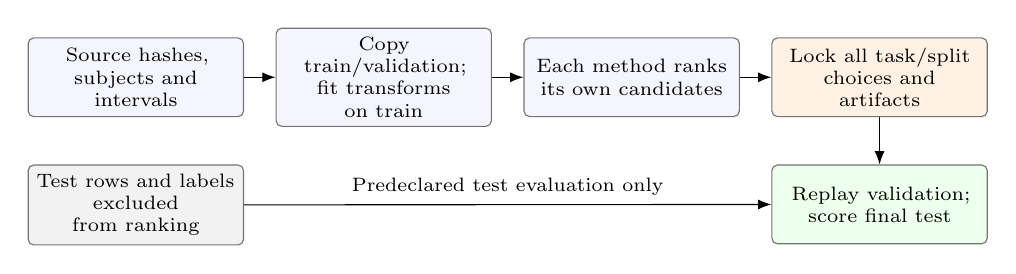
\begin{tikzpicture}[font=\scriptsize,box/.style={draw=black!55,rounded corners=2pt,align=center,minimum height=10mm,text width=25mm,fill=blue!4},>=Latex]
\node[box] (source) {Source hashes,\\subjects and intervals};
\node[box,right=4mm of source] (dev) {Copy train/validation;\\fit transforms on train};
\node[box,right=4mm of dev] (select) {Each method ranks\\its own candidates};
\node[box,right=4mm of select,fill=orange!10] (lock) {Lock all task/split\\choices and artifacts};
\node[box,below=6mm of lock,fill=green!7] (test) {Replay validation;\\score final test};
\node[box,below=6mm of source,fill=gray!10] (hold) {Test rows and labels\\excluded from ranking};
\draw[->] (source)--(dev);\draw[->] (dev)--(select);\draw[->] (select)--(lock);\draw[->] (lock)--(test);
\draw[->] (hold)--node[above,align=center]{Predeclared test evaluation only}(test);
\end{tikzpicture}
\caption{Evaluation flow. Source identifiers determine partitions and audit records but never enter predictive features. The main extension locks all 81 task/split selections; the transfer study separately locks its nine selections.}
\label{fig:flow}
\end{figure}

\subsection{A fixed-mask control with a matched training budget}
A cheaper fixed mask and a selector that trains several masks do not spend the same compute. With $K$ masks and $E=30$ epochs, selection trains $K$ independent JEPA models for $E$ epochs each. Our matched control holds the first mask fixed and trains one model for $KE$ epochs, saving checkpoints at $E,2E,\ldots,KE$. Validation selects among these checkpoints and the same five probe strengths. Both policies spend exactly the same number of optimizer updates and $5K$ probe fits, and use the same architecture, training rows, observation count, and forecast target. The fixed run always finishes its full budget, even if an earlier checkpoint is selected.

This controls optimization steps and validation-choice counts rather than claiming identical measured wall time. The policies necessarily have different initialization/restart and minibatch histories. We also report the first mask after only 30 epochs as a separate, cheaper diagnostic. Its comparison isolates a different question and is not substituted for the matched-budget result.

\section{Experimental protocol}
\subsection{Repeated splits and raw sensor trajectories}
The main extension evaluates 27 tasks on 25 underlying datasets: the prior 23 tasks plus activity classification and forecasting for each of MHEALTH \citep{banos2014mhealth} and PAMAP2 \citep{reiss2012pamap}. This gives 18 classification and nine forecasting tasks. Two outcomes on one sensor corpus are not counted as independent datasets. The prior collection contains 12 public classification datasets, four synthetic classification families, and seven synthetic forecasting families; its source limitations remain documented in Appendix~\ref{app:data}.

MHEALTH supplies 1,600 windows from ten subjects; PAMAP2 supplies 1,280 from eight protocol subjects. Each window contains nine accelerometer channels from three body locations and 64 readings at an effective 50 Hz. MHEALTH readings are consecutive. PAMAP2 retains every second 100-Hz reading without interpolation or antialias filtering. We require finite values, contiguous source samples, and one nonzero activity throughout the entire raw interval. Windows do not overlap. Up to 160 valid windows per subject are sampled without using activity class for balancing. The source-limited PAMAP2 subject 109 is excluded before sampling. Original archive/member hashes, file names, sample bounds and subject IDs accompany every window. PAMAP2 supplies timestamps; MHEALTH time bounds are source-relative row-index/50 estimates, not measured wall-clock times.

Filtering null activities and transitions uses source annotations in both tasks. The forecast population is consequently segmented activities, not unconstrained streaming. Group splits prevent subject overlap, but they cannot remove acquisition bias or make this a clinical validation. The target horizon is 0.32 seconds and all forecasted channels are accelerations in $\mathrm{m/s^2}$.

Data/generation seed is 2026; new split seeds are 4026, 5026, and 6026. Splitting is label-independent and nominally 60/20/20 by whole group where available, otherwise by row. Integer floors give MHEALTH 6/2/2 subjects and PAMAP2 4/2/2. HAR uses supplied subjects; PenDigits uses inferred source groups with a documented identity caveat; synthetic windows stay with their source trajectory. Every split uses neural initialization seed 7. Reported sample SD therefore captures split variation conditional on this initialization. Repeated splits overlap, and reused datasets are not independent external validation.

\subsection{Baselines and compute}
The pilot, its directly supervised online encoder, and TabM each train for 30 epochs per mask with Adam at $10^{-3}$, batches of up to 128, and gradient clipping at 10. Direct supervision uses cross-entropy or training-standardized-target MSE with a linear output head. TabM uses the official package with two width-128 blocks, eight members, dropout 0.1, and numeric inputs without learned numeric embeddings; member losses train the ensemble, and class probabilities are averaged at inference. All methods receive the same observed source coordinates within a candidate, but they use different objectives and parameter counts. Equal epochs across architectures are not equal FLOPs.

Extra Trees uses 100 trees, minimum leaf size two, and validation-selected depths 8/16. CatBoost is classification-only, with 100 iterations, learning rate 0.1, and depths 4/6. Both independently select their masks. Additional feature-selection baselines rank legal training coordinates by ANOVA F (classification), mean squared target correlation (forecasting), or training-fitted Extra Trees importance. Each ranking keeps exactly the common observation count, then fits its own tuned linear or Extra Trees predictor. The ranking fits and finer selection domain are disclosed; these controls are not claimed to have the JEPA policy pair's compute budget.

The main study has 321 mask/split combinations, three neural model families, and 81 extended fixed-mask trajectories: \ExtRuns{} neural training trajectories with \ExtCheckpoints{} saved checkpoint snapshots. Training and encoding use an Apple M3 Max GPU through MPS with fallback disabled. CatBoost, trees, preprocessing, feature ranking and scikit-learn probes \citep{pedregosa2011sklearn} use CPU. Device evidence records parameter, input, loss and gradient placement. Per-run time is retained, but interleaved work on the shared host precludes a controlled hardware-speed comparison.

\subsection{Official I-JEPA/V-JEPA transfer and verification}
The transfer study uses independently sampled 600-image subsets of Digits and Semeion, and 240 generated eight-frame motion clips from 60 simulated entities. Four consecutive clips share an entity and remain in one partition. The four motion laws are horizontal/vertical periodic wrap, circular motion, and horizontal sinusoidal motion. This is a toy visual discrimination problem, not a physical simulator or natural-video benchmark. It uses the same three split seeds and predeclared scratch-model settings.

Official Meta I-JEPA ViT-H/14 ImageNet-1K weights provide frozen image embeddings through Transformers. Official V-JEPA ViT-L/16 VideoMix2M target-encoder weights use pinned native source and eight-frame inference with the official positional interpolation, although pretraining used 16 frames. Both mean-pool patch tokens and fit the same logistic probe grid. Hidden source pixels are zeroed \emph{before} RGB replication and resizing to 224, preventing interpolation from revealing them. The custom video pilot receives the same visible source pixels through its sequence encoder. Pixel budgets match; resizing, architecture and external pretraining compute differ. Fixed pretrained embeddings can be cached without labels; each probe receives only its own split's development rows.

Across the two new studies, 1,392 scratch checkpoint snapshots are replayed on eight training examples each on CPU and MPS, with absolute/relative tolerance $5\times10^{-4}$. All saved test prediction files are independently rescored, and selection rankings, equal-budget constraints and group separation are checked. The local suite passes 173 tests, including test-value poisoning, hidden-pixel noninterference, provenance-window rejection, and lock tampering. The lightweight artifact supplies results, hashes and replay reports; large checkpoints and downloaded archives remain outside it. These checks concern implementation, not model validity or source authenticity.

\section{Results}
\subsection{Selection under matched compute and independent baselines}
The selected-mask policy exceeds the matched-budget fixed mask on \ExtPolicyWins/27 task means and the cheaper 30-epoch fixed mask on \ExtShortWins/27. Against matched compute, selection loses on 16 tasks and ties on one. Thus its majority advantage over the cheaper control disappears when the fixed policy receives the same optimization budget. Figure~\ref{fig:policy} shows paired split differences; bars are sample SDs, not confidence intervals. Table~\ref{tab:counts} summarizes independent model comparisons. JEPA exceeds raw linear on \ExtLinearWins/27, Extra Trees on \ExtTreesWins/27, direct supervision on \ExtSupervisedWins/27, and TabM on \ExtTabMWins/27. CatBoost is evaluated on the 18 classification tasks. These counts use unrounded means; they neither weight datasets by sample size nor establish general superiority.

\begin{table}[t]
\caption{Task means on which JEPA selection is strictly better than each independently selected baseline. Classification uses macro F1; forecasting uses RMSE. Denominators are evaluated tasks, not independent populations. Full mean/SD values appear in Appendix~\ref{app:newresults}.}
\label{tab:counts}\centering\small
\begin{tabular}{lccc}\toprule
Comparison & Classification & Forecasting & All\\\midrule
Fixed mask, matched budget & 9/18 & 1/9 & 10/27\\
Fixed mask, 30 epochs & 13/18 & 3/9 & 16/27\\
Raw linear & 8/18 & 2/9 & 10/27\\
Extra Trees & 2/18 & 3/9 & 5/27\\
Supervised encoder & 3/18 & 1/9 & 4/27\\
TabM & 3/18 & 0/9 & 3/27\\
CatBoost & 3/18 & -- & 3/18\\
Filter + Extra Trees & 3/18 & 4/9 & 7/27\\
Embedded + Extra Trees & 2/18 & 3/9 & 5/27
\\\bottomrule
\end{tabular}
\end{table}

\begin{figure}[t]
\centering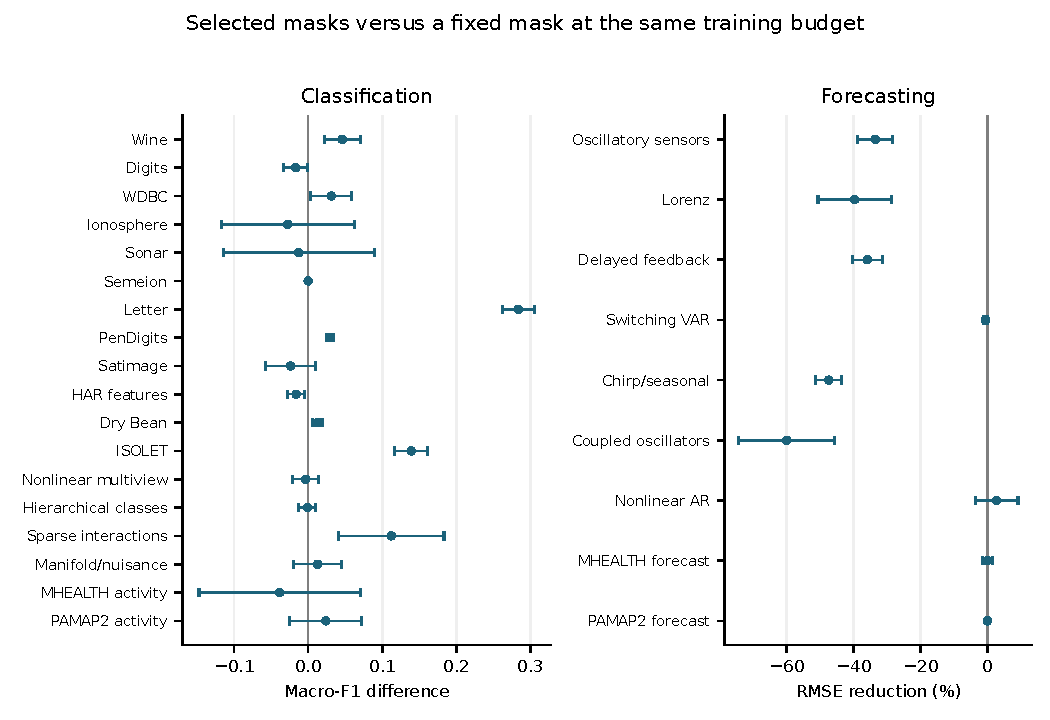
\includegraphics[width=\linewidth]{figures/extension_policy.pdf}
\caption{Selected masks versus a fixed mask with matched optimizer-update and probe-fit budgets. Positive values favor selection. Dots are the mean of three paired split differences and bars are sample SD. Forecast differences use $100(\mathrm{RMSE}_{F}-\mathrm{RMSE}_{J})/\mathrm{RMSE}_{F}$ per split; they are not pooled errors across physical units.}
\label{fig:policy}
\end{figure}

\subsection{Raw sensors and official-model transfer}
Table~\ref{tab:sensors} reports both outcomes for each raw corpus under whole-subject splits. Direct supervision, TabM and Extra Trees outperform JEPA on all four raw-sensor task means; selection exceeds the matched fixed mask only for PAMAP2 activity. These results test generalization across the sampled subjects rather than across overlapping windows from the same subject. The classification and forecasting rows share recordings and should not be treated as four independent data collections. Forecast RMSE aggregates all nine acceleration channels over the fixed future interval; the observation count is 216 scalar values. Activity masks observe 288 scalar values.

\begin{table}[t]
\caption{Raw accelerometer results: mean $\pm$ sample SD over three subject-held-out splits. Activity uses macro F1 ($\uparrow$), forecast uses RMSE in $\mathrm{m/s^2}$ ($\downarrow$). Fixed denotes the matched-budget control. All other methods independently choose their masks.}
\label{tab:sensors}\centering\scriptsize
\begin{tabular}{lccccc}\toprule
Task & JEPA & Fixed & Supervised & TabM & Extra Trees\\\midrule
MHEALTH activity & $0.603\pm0.072$ & $0.641\pm0.038$ & $0.725\pm0.045$ & $0.744\pm0.038$ & $0.791\pm0.090$\\
MHEALTH forecast & $3.971\pm0.410$ & $3.970\pm0.415$ & $3.631\pm0.290$ & $3.516\pm0.319$ & $3.500\pm0.418$\\
PAMAP2 activity & $0.357\pm0.052$ & $0.333\pm0.059$ & $0.388\pm0.140$ & $0.376\pm0.175$ & $0.409\pm0.107$\\
PAMAP2 forecast & $3.644\pm0.609$ & $3.643\pm0.609$ & $3.426\pm0.647$ & $3.240\pm0.599$ & $3.503\pm0.698$
\\\bottomrule
\end{tabular}
\end{table}

\begin{table}[t]
\caption{Visual transfer macro F1, mean $\pm$ sample SD across three splits. Official is frozen I-JEPA for the two 600-image subsets and frozen V-JEPA for synthetic motion. This is an observation-budget comparison with unequal external pretraining compute.}
\label{tab:vision}\centering\small
\begin{tabular}{lcccc}\toprule
Task & JEPA & Supervised & Extra Trees & Official\\\midrule
Digits & $0.808\pm0.016$ & $0.822\pm0.024$ & $0.892\pm0.027$ & $0.915\pm0.043$\\
Semeion & $0.669\pm0.053$ & $0.681\pm0.060$ & $0.690\pm0.076$ & $0.765\pm0.022$\\
Synthetic motion video & $0.404\pm0.029$ & $0.621\pm0.075$ & $0.583\pm0.149$ & $0.771\pm0.091$
\\\bottomrule
\end{tabular}
\end{table}

The official frozen backbone exceeds the small JEPA pilot on all three transfer task means: 0.915 versus 0.808 on Digits, 0.765 versus 0.669 on Semeion, and 0.771 versus 0.404 on synthetic motion. Direct supervision reaches 0.621 on motion, also above the pilot. These results expose limitations of the small representation model; they do not isolate architecture from pretraining. The subsets differ from the main study and are not added to its 27-task win counts. Natural-image/video pretraining, much larger backbones, low-resolution grayscale inputs and resizing all affect transfer. No result here measures official pretraining under the pilot's scratch budget or on raw numeric sensors.

\subsection{Stability, rank, and earlier evidence}
JEPA selects the same named schema mask in all three splits for \ExtStableTasks/27 tasks. Changes across splits are recorded in Appendix~\ref{app:masks}; selection is an empirical development criterion, not a causal feature explanation. For the 321 final candidate embeddings, covariance entropy effective rank has median \ExtRankMedian{}, and \ExtRankFlags/\ExtRankRuns{} have rank below two despite nominal dimension 32. These training-only diagnostics are not ranking inputs. A variance penalty does not ensure high covariance rank; low rank also does not by itself prove that a representation is constant or useless.

The earlier 23-dataset study used 91 masks, three model seeds, 60 epochs, and one split, totaling 273 runs. It exceeded raw linear on 13/23 tasks and Extra Trees on 5/23, with baselines conditioned on JEPA's mask; 198/273 candidates had effective rank below two. We preserve this study in the artifact and Appendix~\ref{app:historical}. Changes in split, epoch budget and baseline selection prevent treating differences between old and new scores as a controlled improvement. The new paired policy comparison supplies the relevant control.

\section{Limitations and responsible use}
The implemented comparisons resolve the earlier absence of direct supervision, specialized tabular baselines, independent feature selection, raw trajectories and repeated group splits within a bounded protocol. Their limits remain substantial. Three repeated partitions with one initialization do not characterize population or joint seed/split uncertainty. Validation is reused for mask/checkpoint and probe selection; there is no nested inner split. Most datasets have been studied previously, some omit entity IDs, and the candidate masks are few and sometimes scientifically arbitrary. The two public sensor corpora contain a small number of volunteers and source-label-filtered activity segments.

Model and tuning budgets are limited. TabM lacks learned numeric embeddings; CatBoost has a small grid and is classification-only. Official visual encoders are frozen transfer baselines, not fully fine-tuned alternatives, and video evidence is synthetic. There is no controlled foundation-model pretraining comparison, natural-video action benchmark, covariance-penalty ablation, intervention, robot rollout, or clinical evaluation. Equal budgets are established for the fixed/search JEPA policy pair as optimizer updates and probe fits; they are not claimed across all model families.

Public historical data and synthetic generation require no new participant recruitment in this work. Source hashes and privacy scans support integrity and reduce accidental disclosure; they do not authenticate collection practices or guarantee privacy. The intended use is research prototyping and evaluation auditing. Safe autonomy, clinical validity, fairness and causal understanding require distinct domain-specific evidence.

\section{Conclusion}
\jepa{} makes observed coordinates, hidden targets, source provenance and selection decisions inspectable. The expanded study compares independently selected baselines, raw subject-held-out sensor tasks, official-model transfer, and a fixed-mask control with a matched training budget. Selection exceeds that control on \ExtPolicyWins/27 task means, while its comparisons with stronger predictors and frequent low rank limit broader claims. The useful outcome is a reproducible way to evaluate both task construction and predictive value without conflating them.

\label{main-end}
\clearpage
\bibliographystyle{plainnat}
\bibliography{references}
\clearpage
\appendix

\section{Complete repeated-split results}\label{app:newresults}
Every entry is mean $\pm$ sample SD over split seeds 4026, 5026 and 6026 with neural seed 7. All methods choose masks independently. Fixed means the fixed-mask trajectory with matched total optimizer updates and probe fits, not the cheaper 30-epoch baseline. Scores are descriptive and not significance tests. Table~\ref{tab:newclass} uses macro F1 and Table~\ref{tab:newforecast} uses original-unit RMSE. Raw feature-selection controls and the cheaper fixed-mask comparison follow.

\begin{table}[h]
\caption{All 18 classification tasks (macro F1, higher is better).}\label{tab:newclass}
\centering\scriptsize\setlength{\tabcolsep}{3pt}
\begin{tabular}{lcccccc}\toprule
Task & JEPA & Fixed & Supervised & TabM & Extra Trees & CatBoost\\\midrule
Wine & $0.914\pm0.055$ & $0.868\pm0.030$ & $0.904\pm0.044$ & $0.913\pm0.031$ & $0.964\pm0.043$ & $0.901\pm0.065$\\
Digits & $0.846\pm0.014$ & $0.862\pm0.005$ & $0.886\pm0.037$ & $0.891\pm0.008$ & $0.887\pm0.025$ & $0.886\pm0.017$\\
WDBC & $0.955\pm0.025$ & $0.924\pm0.007$ & $0.968\pm0.023$ & $0.959\pm0.024$ & $0.946\pm0.022$ & $0.936\pm0.031$\\
Ionosphere & $0.812\pm0.014$ & $0.840\pm0.084$ & $0.860\pm0.023$ & $0.870\pm0.037$ & $0.872\pm0.020$ & $0.846\pm0.053$\\
Sonar & $0.708\pm0.077$ & $0.721\pm0.037$ & $0.743\pm0.052$ & $0.711\pm0.108$ & $0.792\pm0.058$ & $0.799\pm0.066$\\
Semeion & $0.771\pm0.017$ & $0.771\pm0.017$ & $0.844\pm0.022$ & $0.822\pm0.007$ & $0.840\pm0.027$ & $0.829\pm0.021$\\
Letter & $0.652\pm0.011$ & $0.368\pm0.031$ & $0.646\pm0.019$ & $0.709\pm0.020$ & $0.811\pm0.001$ & $0.775\pm0.009$\\
PenDigits & $0.891\pm0.009$ & $0.861\pm0.008$ & $0.925\pm0.008$ & $0.935\pm0.007$ & $0.926\pm0.008$ & $0.929\pm0.004$\\
Satimage & $0.793\pm0.019$ & $0.816\pm0.018$ & $0.806\pm0.004$ & $0.824\pm0.014$ & $0.856\pm0.014$ & $0.842\pm0.015$\\
HAR features & $0.765\pm0.017$ & $0.781\pm0.019$ & $0.918\pm0.009$ & $0.931\pm0.020$ & $0.899\pm0.034$ & $0.901\pm0.002$\\
Dry Bean & $0.927\pm0.008$ & $0.915\pm0.012$ & $0.915\pm0.013$ & $0.927\pm0.010$ & $0.918\pm0.012$ & $0.920\pm0.008$\\
ISOLET & $0.696\pm0.023$ & $0.557\pm0.019$ & $0.912\pm0.013$ & $0.935\pm0.004$ & $0.920\pm0.004$ & $0.890\pm0.011$\\
Nonlinear multiview & $0.871\pm0.022$ & $0.875\pm0.016$ & $0.948\pm0.006$ & $0.949\pm0.008$ & $0.914\pm0.007$ & $0.906\pm0.009$\\
Hierarchical classes & $0.962\pm0.009$ & $0.963\pm0.004$ & $0.968\pm0.006$ & $0.962\pm0.010$ & $0.970\pm0.007$ & $0.970\pm0.009$\\
Sparse interactions & $0.705\pm0.010$ & $0.593\pm0.063$ & $0.895\pm0.010$ & $0.929\pm0.012$ & $0.860\pm0.008$ & $0.930\pm0.009$\\
Manifold/nuisance & $0.856\pm0.035$ & $0.843\pm0.018$ & $0.967\pm0.012$ & $0.959\pm0.008$ & $0.958\pm0.015$ & $0.955\pm0.003$\\
MHEALTH activity & $0.603\pm0.072$ & $0.641\pm0.038$ & $0.725\pm0.045$ & $0.744\pm0.038$ & $0.791\pm0.090$ & $0.797\pm0.067$\\
PAMAP2 activity & $0.357\pm0.052$ & $0.333\pm0.059$ & $0.388\pm0.140$ & $0.376\pm0.175$ & $0.409\pm0.107$ & $0.422\pm0.123$
\\\bottomrule
\end{tabular}
\end{table}
\begin{table}[h]
\caption{All nine forecasting tasks (RMSE, lower is better). Units differ between synthetic generators and raw accelerometers; no cross-task RMSE average is meaningful.}\label{tab:newforecast}
\centering\scriptsize
\begin{tabular}{lccccc}\toprule
Task & JEPA & Fixed & Supervised & TabM & Extra Trees\\\midrule
Oscillatory sensors & $0.294\pm0.004$ & $0.220\pm0.006$ & $0.218\pm0.016$ & $0.235\pm0.017$ & $0.301\pm0.018$\\
Lorenz & $0.926\pm0.044$ & $0.666\pm0.057$ & $0.558\pm0.047$ & $0.892\pm0.046$ & $0.577\pm0.033$\\
Delayed feedback & $0.115\pm0.004$ & $0.084\pm0.005$ & $0.091\pm0.006$ & $0.093\pm0.006$ & $0.093\pm0.004$\\
Switching VAR & $0.178\pm0.004$ & $0.177\pm0.005$ & $0.181\pm0.005$ & $0.176\pm0.004$ & $0.176\pm0.004$\\
Chirp/seasonal & $0.256\pm0.002$ & $0.174\pm0.003$ & $0.159\pm0.006$ & $0.163\pm0.004$ & $0.210\pm0.007$\\
Coupled oscillators & $0.151\pm0.026$ & $0.096\pm0.025$ & $0.050\pm0.003$ & $0.071\pm0.003$ & $0.154\pm0.048$\\
Nonlinear AR & $0.106\pm0.006$ & $0.110\pm0.003$ & $0.102\pm0.004$ & $0.102\pm0.003$ & $0.120\pm0.007$\\
MHEALTH forecast & $3.971\pm0.410$ & $3.970\pm0.415$ & $3.631\pm0.290$ & $3.516\pm0.319$ & $3.500\pm0.418$\\
PAMAP2 forecast & $3.644\pm0.609$ & $3.643\pm0.609$ & $3.426\pm0.647$ & $3.240\pm0.599$ & $3.503\pm0.698$
\\\bottomrule
\end{tabular}
\end{table}
\FloatBarrier

\begin{table}[h]
\caption{Independent feature-selection controls. Linear selects its own schema mask. Filter uses training-only ANOVA F or squared correlation; embedded uses training-only tree importance. Each retains the common scalar observation count. Arrows mark macro F1 ($\uparrow$) or RMSE ($\downarrow$).}
\centering\scriptsize
\begin{tabular}{lccccc}\toprule
Task & Linear & Filter+linear & Embedded+linear & Filter+trees & Embedded+trees\\\midrule
Wine ($\uparrow$) & $0.917\pm0.052$ & $0.942\pm0.026$ & $0.944\pm0.030$ & $0.972\pm0.030$ & $0.980\pm0.034$\\
Digits ($\uparrow$) & $0.865\pm0.016$ & $0.943\pm0.006$ & $0.949\pm0.001$ & $0.960\pm0.004$ & $0.974\pm0.010$\\
Oscillatory sensors ($\downarrow$) & $0.231\pm0.003$ & $0.227\pm0.003$ & $0.221\pm0.010$ & $0.333\pm0.031$ & $0.303\pm0.013$\\
WDBC ($\uparrow$) & $0.962\pm0.011$ & $0.955\pm0.022$ & $0.955\pm0.022$ & $0.949\pm0.017$ & $0.949\pm0.017$\\
Ionosphere ($\uparrow$) & $0.762\pm0.053$ & $0.768\pm0.046$ & $0.766\pm0.045$ & $0.879\pm0.042$ & $0.883\pm0.036$\\
Sonar ($\uparrow$) & $0.691\pm0.103$ & $0.767\pm0.074$ & $0.775\pm0.058$ & $0.797\pm0.047$ & $0.809\pm0.046$\\
Semeion ($\uparrow$) & $0.763\pm0.034$ & $0.879\pm0.015$ & $0.885\pm0.001$ & $0.884\pm0.034$ & $0.895\pm0.019$\\
Letter ($\uparrow$) & $0.611\pm0.019$ & $0.623\pm0.009$ & $0.623\pm0.009$ & $0.813\pm0.019$ & $0.813\pm0.019$\\
PenDigits ($\uparrow$) & $0.824\pm0.005$ & $0.839\pm0.019$ & $0.874\pm0.017$ & $0.918\pm0.013$ & $0.920\pm0.015$\\
Satimage ($\uparrow$) & $0.772\pm0.027$ & $0.819\pm0.007$ & $0.811\pm0.020$ & $0.873\pm0.011$ & $0.873\pm0.013$\\
HAR features ($\uparrow$) & $0.946\pm0.010$ & $0.921\pm0.024$ & $0.919\pm0.013$ & $0.890\pm0.019$ & $0.919\pm0.011$\\
Dry Bean ($\uparrow$) & $0.927\pm0.008$ & $0.919\pm0.013$ & $0.909\pm0.014$ & $0.900\pm0.009$ & $0.887\pm0.009$\\
ISOLET ($\uparrow$) & $0.929\pm0.003$ & $0.926\pm0.008$ & $0.937\pm0.006$ & $0.919\pm0.012$ & $0.930\pm0.011$\\
Lorenz ($\downarrow$) & $2.504\pm0.045$ & $2.563\pm0.039$ & $2.498\pm0.040$ & $0.569\pm0.030$ & $0.575\pm0.032$\\
Delayed feedback ($\downarrow$) & $0.094\pm0.005$ & $0.098\pm0.003$ & $0.095\pm0.003$ & $0.099\pm0.004$ & $0.100\pm0.004$\\
Switching VAR ($\downarrow$) & $0.178\pm0.004$ & $0.179\pm0.004$ & $0.179\pm0.004$ & $0.176\pm0.004$ & $0.176\pm0.004$\\
Chirp/seasonal ($\downarrow$) & $0.172\pm0.003$ & $0.175\pm0.007$ & $0.168\pm0.003$ & $0.210\pm0.008$ & $0.200\pm0.008$\\
Coupled oscillators ($\downarrow$) & $0.039\pm0.003$ & $0.039\pm0.004$ & $0.038\pm0.004$ & $0.153\pm0.048$ & $0.154\pm0.047$\\
Nonlinear AR ($\downarrow$) & $0.100\pm0.004$ & $0.137\pm0.008$ & $0.099\pm0.004$ & $0.151\pm0.019$ & $0.119\pm0.008$\\
Nonlinear multiview ($\uparrow$) & $0.868\pm0.008$ & $0.875\pm0.011$ & $0.874\pm0.011$ & $0.912\pm0.006$ & $0.915\pm0.006$\\
Hierarchical classes ($\uparrow$) & $0.963\pm0.006$ & $0.960\pm0.003$ & $0.963\pm0.013$ & $0.952\pm0.001$ & $0.970\pm0.002$\\
Sparse interactions ($\uparrow$) & $0.911\pm0.013$ & $0.952\pm0.009$ & $0.952\pm0.009$ & $0.883\pm0.013$ & $0.870\pm0.023$\\
Manifold/nuisance ($\uparrow$) & $0.910\pm0.006$ & $0.941\pm0.015$ & $0.938\pm0.014$ & $0.972\pm0.008$ & $0.976\pm0.003$\\
MHEALTH activity ($\uparrow$) & $0.694\pm0.019$ & $0.648\pm0.031$ & $0.720\pm0.049$ & $0.806\pm0.086$ & $0.802\pm0.087$\\
MHEALTH forecast ($\downarrow$) & $3.828\pm0.394$ & $4.182\pm0.392$ & $3.720\pm0.353$ & $3.592\pm0.398$ & $3.474\pm0.398$\\
PAMAP2 activity ($\uparrow$) & $0.323\pm0.117$ & $0.376\pm0.070$ & $0.337\pm0.126$ & $0.442\pm0.084$ & $0.421\pm0.117$\\
PAMAP2 forecast ($\downarrow$) & $3.343\pm0.483$ & $3.726\pm0.644$ & $3.324\pm0.449$ & $3.764\pm0.661$ & $3.505\pm0.680$
\\\bottomrule
\end{tabular}
\end{table}
\FloatBarrier
\begin{table}[h]
\caption{The cheaper fixed mask and matched-budget fixed mask answer different comparisons. Both use the first schema mask. The matched trajectory finishes $30K$ epochs and validation chooses one of $K$ checkpoints. Arrows mark macro F1 ($\uparrow$) or RMSE ($\downarrow$).}
\centering\small
\begin{tabular}{lccc}\toprule
Task & Selected masks & Fixed, 30 epochs & Fixed, matched budget\\\midrule
Wine ($\uparrow$) & $0.914\pm0.055$ & $0.871\pm0.028$ & $0.868\pm0.030$\\
Digits ($\uparrow$) & $0.846\pm0.014$ & $0.848\pm0.011$ & $0.862\pm0.005$\\
Oscillatory sensors ($\downarrow$) & $0.294\pm0.004$ & $0.299\pm0.010$ & $0.220\pm0.006$\\
WDBC ($\uparrow$) & $0.955\pm0.025$ & $0.915\pm0.021$ & $0.924\pm0.007$\\
Ionosphere ($\uparrow$) & $0.812\pm0.014$ & $0.763\pm0.013$ & $0.840\pm0.084$\\
Sonar ($\uparrow$) & $0.708\pm0.077$ & $0.662\pm0.026$ & $0.721\pm0.037$\\
Semeion ($\uparrow$) & $0.771\pm0.017$ & $0.771\pm0.017$ & $0.771\pm0.017$\\
Letter ($\uparrow$) & $0.652\pm0.011$ & $0.324\pm0.028$ & $0.368\pm0.031$\\
PenDigits ($\uparrow$) & $0.891\pm0.009$ & $0.828\pm0.030$ & $0.861\pm0.008$\\
Satimage ($\uparrow$) & $0.793\pm0.019$ & $0.780\pm0.015$ & $0.816\pm0.018$\\
HAR features ($\uparrow$) & $0.765\pm0.017$ & $0.763\pm0.008$ & $0.781\pm0.019$\\
Dry Bean ($\uparrow$) & $0.927\pm0.008$ & $0.896\pm0.014$ & $0.915\pm0.012$\\
ISOLET ($\uparrow$) & $0.696\pm0.023$ & $0.507\pm0.007$ & $0.557\pm0.019$\\
Lorenz ($\downarrow$) & $0.926\pm0.044$ & $0.926\pm0.044$ & $0.666\pm0.057$\\
Delayed feedback ($\downarrow$) & $0.115\pm0.004$ & $0.115\pm0.004$ & $0.084\pm0.005$\\
Switching VAR ($\downarrow$) & $0.178\pm0.004$ & $0.178\pm0.004$ & $0.177\pm0.005$\\
Chirp/seasonal ($\downarrow$) & $0.256\pm0.002$ & $0.256\pm0.002$ & $0.174\pm0.003$\\
Coupled oscillators ($\downarrow$) & $0.151\pm0.026$ & $0.152\pm0.026$ & $0.096\pm0.025$\\
Nonlinear AR ($\downarrow$) & $0.106\pm0.006$ & $0.112\pm0.000$ & $0.110\pm0.003$\\
Nonlinear multiview ($\uparrow$) & $0.871\pm0.022$ & $0.873\pm0.010$ & $0.875\pm0.016$\\
Hierarchical classes ($\uparrow$) & $0.962\pm0.009$ & $0.963\pm0.004$ & $0.963\pm0.004$\\
Sparse interactions ($\uparrow$) & $0.705\pm0.010$ & $0.589\pm0.034$ & $0.593\pm0.063$\\
Manifold/nuisance ($\uparrow$) & $0.856\pm0.035$ & $0.791\pm0.020$ & $0.843\pm0.018$\\
MHEALTH activity ($\uparrow$) & $0.603\pm0.072$ & $0.616\pm0.022$ & $0.641\pm0.038$\\
MHEALTH forecast ($\downarrow$) & $3.971\pm0.410$ & $3.938\pm0.391$ & $3.970\pm0.415$\\
PAMAP2 activity ($\uparrow$) & $0.357\pm0.052$ & $0.342\pm0.070$ & $0.333\pm0.059$\\
PAMAP2 forecast ($\downarrow$) & $3.644\pm0.609$ & $3.614\pm0.644$ & $3.643\pm0.609$
\\\bottomrule
\end{tabular}
\end{table}
\FloatBarrier

\section{Selected masks across splits}\label{app:masks}
The exact indices and independent choices for every method are in the machine-readable locks. Names below summarize JEPA's choices only. They are not feature-importance claims.
\begin{table}[h]
\caption{JEPA schema-mask selections across the three repeated splits.}\centering\scriptsize
\begin{tabular}{llll}\toprule
Task & Split 4026 & Split 5026 & Split 6026\\\midrule
Wine & alternating\_columns & last\_columns & alternating\_columns\\
Digits & top\_half & top\_half & bottom\_half\\
Oscillatory sensors & recent\_past & recent\_past & spaced\_past\\
WDBC & worst\_measurements & worst\_measurements & worst\_measurements\\
Ionosphere & alternating\_tokens & alternating\_tokens & alternating\_tokens\\
Sonar & alternating\_tokens & first\_tokens & first\_tokens\\
Semeion & left\_half & left\_half & left\_half\\
Letter & last\_columns & last\_columns & last\_columns\\
PenDigits & alternating\_tokens & alternating\_tokens & alternating\_tokens\\
Satimage & bands\_0\_2 & bands\_1\_3 & bands\_1\_3\\
HAR features & last\_columns & alternating\_columns & alternating\_columns\\
Dry Bean & last\_columns & last\_columns & last\_columns\\
ISOLET & middle\_columns & alternating\_columns & last\_columns\\
Lorenz & recent\_past & recent\_past & recent\_past\\
Delayed feedback & recent\_past & recent\_past & recent\_past\\
Switching VAR & recent\_past & recent\_past & recent\_past\\
Chirp/seasonal & recent\_past & recent\_past & recent\_past\\
Coupled oscillators & spaced\_past & recent\_past & recent\_past\\
Nonlinear AR & spaced\_past & spaced\_past & spaced\_past\\
Nonlinear multiview & middle\_columns & alternating\_columns & first\_columns\\
Hierarchical classes & first\_columns & last\_columns & alternating\_columns\\
Sparse interactions & alternating\_columns & alternating\_columns & alternating\_columns\\
Manifold/nuisance & alternating\_columns & alternating\_columns & alternating\_columns\\
MHEALTH activity & alternating\_tokens & last\_tokens & last\_tokens\\
MHEALTH forecast & recent\_past & middle\_past & spaced\_past\\
PAMAP2 activity & alternating\_tokens & alternating\_tokens & alternating\_tokens\\
PAMAP2 forecast & recent\_past & recent\_past & spaced\_past
\\\bottomrule
\end{tabular}
\end{table}
\FloatBarrier

\section{Data provenance and sampling}\label{app:data}
The original public collection includes Wine, Digits, WDBC, Ionosphere, Sonar, Semeion, Letter, PenDigits, Satimage, HAR, Dry Bean and ISOLET. Their retained samples, feature engineering and new partitions are not original benchmark protocols. UCI source records and the artifact provide attribution; numeric sources are labeled CC BY 4.0 by UCI. Synthetic generators are designated CC0-1.0. Original prototype code uses Apache-2.0; official pretrained weight licenses are recorded separately.

\begin{table}[h]
\caption{Primary UCI dataset identifiers.}\centering\small
\begin{tabular}{ll@{\qquad}ll}\toprule
Dataset & DOI & Dataset & DOI\\\midrule
Wine & 10.24432/C5PC7J & Digits & 10.24432/C50P49\\
WDBC & 10.24432/C5DW2B & Ionosphere & 10.24432/C5W01B\\
Sonar & 10.24432/C5T01Q & Semeion & 10.24432/C5SC8V\\
Letter & 10.24432/C5ZP40 & PenDigits & 10.24432/C5MG6K\\
Satimage & 10.24432/C55887 & HAR & 10.24432/C54S4K\\
Dry Bean & 10.24432/C50S4B & ISOLET & 10.24432/C51G69\\
MHEALTH & 10.24432/C5TW22 & PAMAP2 & 10.24432/C5NW2H\\\bottomrule
\end{tabular}
\end{table}

The downloaded adapters remove exact duplicate feature vectors before sampling (one Ionosphere, 1,332 Letter and 68 Dry Bean records; none in the other downloaded sources). Ungrouped collections above 3,000 unique rows are sampled without replacement at seed 2026. HAR retains 100 records per explicit subject, totaling 3,000. PenDigits retains 68 per source group, totaling 2,992, using the second field of aligned UNIPEN comments under separate original train/test namespaces. This follows source structure and donor group counts, not independently verified writer identity. Where provided, original source partitions are pooled before the new split.

HAR contains source-engineered, normalized features, so our training-only normalization does not undo upstream preprocessing. ISOLET, Semeion and Satimage omit explicit speaker, writer or geographic fields needed to establish those independence claims. Raw MHEALTH/PAMAP2 windows instead preserve source sample bounds and subject grouping. Activity and forecasting outcomes on each raw corpus use the same selected windows. ECG, heart rate, demographics and subject identifiers are not model features. Macro F1 uses the standard observed/predicted-class union; rare classes can be absent from a partition, and class coverage can differ across held-out subject sets.

The seven prior synthetic forecasts cover oscillatory sensors, Lorenz trajectories, delayed feedback inspired by Mackey--Glass, switching vector autoregression, chirp/seasonal components, coupled oscillators and nonlinear autoregression. Four synthetic classifications cover nonlinear multiview structure, hierarchical classes, sparse interactions and manifold/nuisance variables. Equations and seeds are supplied in source; the delayed-feedback case is not a canonical Mackey--Glass benchmark replication. The new visual generator renders noisy Gaussian shapes under four seeded kinematic laws, with consecutive clips grouped by entity.

\section{Implementation and reproducibility}\label{app:implementation}
For covariance eigenvalues $\lambda_j\geq0$, the entropy effective rank is $\exp(-\sum_{j:p_j>0}p_j\log p_j)$, where $p_j=\lambda_j/\sum_\ell\lambda_\ell$; it is zero if total variance is zero. Diagnostics use training embeddings and do not affect selection.

The tabular encoder maps $2d$ value/mask inputs through widths 64, 64 and 32 with GELU hidden activations. The image network uses 3-by-3 convolutions (16 then 32 channels, padding one), flattening, and a 64-to-32 head. The sequence network uses 32-channel convolutions with kernels five and three (padding two and one), flattening, and the same head. The predictor is 32-to-64-to-32 with hidden GELU. Direct supervision replaces the predictor with a task-output linear head and optimizes the online encoder and head against labels or future coordinates. Forecast targets are standardized on training data for neural supervised loss, then returned to original units for metrics.

TabM uses package 0.0.3 and CatBoost 1.2.10. The official I-JEPA revision is \texttt{f157467ea509bc356ff9\allowbreak{}f61fd3c0d840eec5e04e}; the native V-JEPA source revision is \texttt{51c59d518fc63c08464a\allowbreak{}f6de585f78ac0c7ed4d5}. Checkpoint hashes and exact processor/device settings are in the result payload. I-JEPA uses its published processor (including normalization); V-JEPA uses explicit bilinear resizing and ImageNet channel normalization without cropping. Grayscale-to-RGB replication introduces no additional source observation. Official backbones remain frozen; the reported downstream head is logistic regression, not the official attentive-probe recipe.

The MPS runs record actual device placement and reject fallback. Replay checks verify \ExtCheckpoints{} main and \VisionCheckpoints{} transfer scratch checkpoint snapshots against CPU inference on eight training rows each, and rescore every saved test prediction. The reported tolerance is absolute/relative $5\times10^{-4}$; this is not a bitwise portability guarantee. Constant-feature warnings in filter ranking are handled deterministically; nonfinite rankings are placed last. Warnings and study-specific checks accompany the artifact rather than silently excluding candidates.

\begin{verbatim}
python -m pip install '.[dev,report,experiments]'
PYTHONPATH=src python scripts/run_extension.py \
  --config configs/extension.json --output artifacts/new_extension
PYTHONPATH=src python scripts/validate_extension.py \
  --directory artifacts/new_extension
PYTHONPATH=src python scripts/run_vision_transfer.py \
  --output artifacts/new_vision
PYTHONPATH=src python scripts/validate_extension.py \
  --directory artifacts/new_vision --vision
PYTHONPATH=src python paper/neurips2026/build_extension_evidence.py
\end{verbatim}
Fresh output directories preserve frozen evidence. Public sources download into ignored local caches. Official weights are not redistributed. To regenerate paper tables without GPU retraining, run the builder against the supplied frozen \texttt{results/} payloads and their validation reports. Those reports attest to the recorded local replay; the lightweight archive cannot independently replay checkpoints that it does not include.

\section{Historical 273-run study}\label{app:historical}
This earlier study used split seed 3026, model seeds 7/17/27, and 60 epochs per candidate. Its 91 masks were all selected and locked before test scoring. Unlike the extension, raw linear, PCA, Extra Trees and random-encoder baselines were evaluated on JEPA's selected context. Mean/sample SD below describe model initialization on one split, not split variation. These results are retained for continuity and are not pooled with the new comparisons.

\begin{table}[h]
\caption{Historical classification macro F1 under a JEPA-selected observation mask.}\centering\small
\begin{tabular}{lrccc}\toprule
Dataset & $|C|$ & JEPA + linear & Raw linear & Extra Trees\\\midrule
Wine & 6 & 0.899 $\pm$ 0.015 & 0.891 $\pm$ 0.000 & 0.936 $\pm$ 0.014 \\
Digits & 32 & 0.883 $\pm$ 0.022 & 0.857 $\pm$ 0.000 & 0.902 $\pm$ 0.011 \\
Breast Cancer & 10 & 0.969 $\pm$ 0.005 & 0.963 $\pm$ 0.000 & 0.953 $\pm$ 0.009 \\
Ionosphere & 16 & 0.897 $\pm$ 0.036 & 0.883 $\pm$ 0.000 & 0.978 $\pm$ 0.010 \\
Sonar & 30 & 0.730 $\pm$ 0.014 & 0.712 $\pm$ 0.000 & 0.776 $\pm$ 0.014 \\
Semeion & 128 & 0.754 $\pm$ 0.013 & 0.768 $\pm$ 0.000 & 0.824 $\pm$ 0.009 \\
Letter & 8 & 0.665 $\pm$ 0.036 & 0.598 $\pm$ 0.000 & 0.823 $\pm$ 0.004 \\
PenDigits & 8 & 0.904 $\pm$ 0.002 & 0.807 $\pm$ 0.000 & 0.948 $\pm$ 0.004 \\
Satimage & 18 & 0.828 $\pm$ 0.007 & 0.766 $\pm$ 0.000 & 0.874 $\pm$ 0.004 \\
HAR & 280 & 0.785 $\pm$ 0.024 & 0.946 $\pm$ 0.000 & 0.895 $\pm$ 0.008 \\
Dry Bean & 8 & 0.918 $\pm$ 0.005 & 0.926 $\pm$ 0.000 & 0.916 $\pm$ 0.006 \\
ISOLET & 308 & 0.764 $\pm$ 0.012 & 0.943 $\pm$ 0.000 & 0.932 $\pm$ 0.012 \\
Multiview factors & 32 & 0.881 $\pm$ 0.005 & 0.840 $\pm$ 0.000 & 0.907 $\pm$ 0.010 \\
Hierarchical classes & 40 & 0.968 $\pm$ 0.006 & 0.965 $\pm$ 0.000 & 0.968 $\pm$ 0.006 \\
Sparse interactions & 48 & 0.730 $\pm$ 0.007 & 0.907 $\pm$ 0.000 & 0.867 $\pm$ 0.012 \\
Manifold + nuisance & 48 & 0.807 $\pm$ 0.047 & 0.773 $\pm$ 0.000 & 0.973 $\pm$ 0.004 
\\\bottomrule
\end{tabular}
\end{table}
\begin{table}[h]
\caption{Historical synthetic forecasting RMSE under a JEPA-selected observation mask.}\centering\small
\begin{tabular}{lrccc}\toprule
Dataset & $|C|$ & JEPA + linear & Raw linear & Extra Trees\\\midrule
Sensor oscillator & 18 & 0.276 $\pm$ 0.017 & 0.239 $\pm$ 0.000 & 0.351 $\pm$ 0.003 \\
Lorenz & 36 & 0.754 $\pm$ 0.034 & 2.500 $\pm$ 0.000 & 0.617 $\pm$ 0.005 \\
Delayed dynamics & 36 & 0.083 $\pm$ 0.002 & 0.079 $\pm$ 0.000 & 0.082 $\pm$ 0.001 \\
Switching VAR & 48 & 0.178 $\pm$ 0.001 & 0.180 $\pm$ 0.000 & 0.177 $\pm$ 0.000 \\
Chirp-seasonal & 36 & 0.226 $\pm$ 0.021 & 0.191 $\pm$ 0.000 & 0.220 $\pm$ 0.001 \\
Coupled oscillators & 48 & 0.109 $\pm$ 0.016 & 0.035 $\pm$ 0.000 & 0.135 $\pm$ 0.001 \\
Nonlinear AR & 36 & 0.098 $\pm$ 0.001 & 0.094 $\pm$ 0.000 & 0.114 $\pm$ 0.000 
\\\bottomrule
\end{tabular}
\end{table}
\FloatBarrier
The original frozen payload, other baselines, inventory, all candidate rankings and the original replay report remain in the artifact. All 273 historical checkpoints and validation probes were replayed, with maximum CPU/MPS embedding difference $1.34\times10^{-5}$ at absolute/relative tolerance $10^{-4}$. The old 169-test report is historical evidence; the current expanded suite has 173 passing local tests. An earlier 138-run fixed-policy pilot is excluded from both comparisons because its masks and splits differ.

\section{AI assistance and author responsibility}
An AI assistant supported implementation, experiment orchestration, analysis and writing. It is neither an author nor a component of the predictor or ranking rule. Human authors must review the scientific claims, references, authorship, disclosures and workshop requirements before submitting this draft. No submission, acceptance, funding award or institutional ethics approval is implied.
\end{document}
